
\جزوحصہ{سطح حرکت پر ایک درجی مساوات میں تبادلہ}
سطح حرکت کی دوسری ترکیب خود مختار [جس میں \عددیء{t} صریحاً نہیں پایا جاتا] دو درجی سادہ تفرقی مساوات
\begin{align*}
F(y,y',y'')=0
\end{align*}
میں \عددی{y=y_1} کو آزاد متغیرہ اور \عددی{y'=y_2} لے کر \عددی{y''} کو زنجیری تفرق سے
\begin{align*}
y''=y_2'=\frac{\dif y_2}{\dif t}=\frac{\dif y_2}{\dif y_1}\frac{\dif y_1}{\dif t}=\frac{\dif y_2}{\dif y_1}y_2
\end{align*}
لکھ کر ایک درجی مساوات
\begin{align}
F\left(y_1,y_2,\frac{\dif y_2}{\dif y_1}y_2\right)=0
\end{align}
میں تبدیل کرنے پر مبنی ہے۔اس ایک درجی مساوات کو یا تو حل کرنا ممکن ہوتا ہے اور یا \اصطلاح{میدان ڈھال}\فرہنگ{میدان!ڈھال}\فرہنگ{ڈھال!میدان} کی مدد سے اس پر غور ممکن ہوتا ہے۔ آئیں مثال \حوالہ{مثال_نظام_دھاگے_سے_لٹکی_کمیت} پر اس ترکیب کی مدد سے غور کریں۔
%==========

\ابتدا{مثال}\شناخت{مثال_نظام_بلا_تقصیر_ارتعاش_یک_درجی_مساوات}\quad بلا تقصیر ارتعاشی نظام کی ایک درجی تفرقی مساوات۔\\
مساوات \حوالہ{مساوات_نظام_غیر_خطی_ترکیب_مرحلہ_ت} میں \عددی{\theta''+k\sin \theta=0} ہے جس میں \عددی{\theta=y_1} اور  \عددی{\theta'=y_2} (زاویائی رفتار) لیتے ہوئے
\begin{align*}
\theta''=\frac{\dif y_2}{\dif t}=\frac{\dif y_2}{\dif y_1}\frac{\dif y_1}{\dif t}=\frac{\dif y_2}{\dif y_1}y_2
\end{align*}
لکھ کر \عددی{\tfrac{\dif y_2}{\dif y_1}y_2=-k\sin y_1} ملتا ہے جس کو علیحدگی متغیرات سے \عددی{y_2\dif y_2=-k\sin y_1\dif y_1} لکھا جا سکتا ہے جس کا تکمل
\begin{align}\label{مساوات_نظام_کل_توانائی_الف}
\frac{1}{2}y_2^2=k\cos y_1+C 
\end{align}
دیتا ہے جہاں \عددی{C} تکمل کا مستقل ہے۔اس کو \عددی{mL^2} سے ضرب دینے سے
\begin{align*}
\frac{1}{2}m(Ly_2)^2-mL^2k\cos y_1=mL^2C
\end{align*}
حاصل ہوتا ہے جس کے تینوں اجزاء \اصطلاح{توانائی}\فرہنگ{توانائی}\حاشیہب{energy}\فرہنگ{energy} کو ظاہر کرتے ہیں۔چونکہ \عددی{y_2} زاویائی رفتار ہے لہٰذا \عددی{Ly_2} لمحاتی رفتار اور  \عددی{\tfrac{1}{2}m(Ly_2)^2} \اصطلاح{حرکی توانائی}\فرہنگ{حرکی توانائی}\فرہنگ{توانائی!حرکی}\حاشیہب{kinetic energy}\فرہنگ{energy!kinetic} ہے۔درج بالا مساوات کا دوسرا جزو (بمع منفی علامت) \اصطلاح{مخفی توانائی}\فرہنگ{توانائی!مخفی}\فرہنگ{مخفی توانائی}\حاشیہب{potential energy}\فرہنگ{energy!potential} ہے جبکہ مساوات کا دایاں ہاتھ \عددی{mL^2C} کل توانائی ہے۔بلا تقصیر نظام میں توانائی کا ضیاع نہیں پایا جاتا لہٰذا حزب توقع کل توانائی مستقل مقدار ہے۔آئیں دیکھیں کہ حرکت کی نوعیت کل توانائی پر کیسے منحصر ہے۔

شکل \حوالہ{شکل_مثال_نظام_دھاگے_سے_لٹکی_کمیت}-ب مختلف \عددی{C} کے لئے خط حرکت دیتی ہے۔ان خطوط کا دوری عرصہ \عددی{2\pi} ہے۔ان میں ترخیمی بند دائرے اور  لہر نما خطوط شامل ہیں جن کے مابین نقطہ زین [\عددی{(n\pi,0)} جہاں \عددی{n=\mp1,\mp3,\cdots} ہے] سے گزرتے ہوئے دو عدد خط حرکت  پائے جاتے ہیں۔مساوات \حوالہ{مساوات_نظام_کل_توانائی_الف} کے تحت \عددی{C} کی کم سے کم قیمت \عددی{C=-k} ہے جس پر \عددی{y_2=0} اور \عددی{\cos y_1=1} ہوں گے جو ساکن کمیت کو ظاہر کرتی ہے۔جس نقطے پر \عددی{y_2=\theta'=0} ہو اس نقطے پر حرت کی سمت تبدیل ہو کر الٹ ہو جائے گی لہٰذا مساوات \حوالہ{مساوات_نظام_کل_توانائی_الف} میں \عددی{y_2=0} پر کرتے ہوئے \عددی{k\cos y_1+C=0} حاصل ہوتا ہے۔اب اگر \عددی{y_1=\pi} ہو تب \عددی{\cos y_1=-1} اور یوں \عددی{C=k} ہو گا۔اس طرح اگر \عددی{-k<C<k} ہو تب \عددی{\abs{y_1}=\abs{\theta}<\pi} کی صورت میں کمیت کی حرکت کی سمت الٹ ہو گی اور \عددی{C} کی ان قیمتوں \عددی{(\abs{C}<k)} کے لئے کمیت ارتیاش پذیر ہو گا۔ترخیمی بند دائرے اس ارتعاشی حرکت کو ظاہر کرتے ہیں۔اس کے برعکس \عددی{C>k} کی صورت میں \عددی{y_2=0} ممکن نہیں ہے لہٰذا کمیت کی حرکت کی سمت الٹ نہیں ہو گی لہٰذا کمیت مرکز کے گرد گھومتا رہے گا جس کو لہری خط حرکت ظاہر کرتی ہیں۔ان دو صورتوں کے مابین \عددی{C=k} پایا جاتا ہے جس کے خطوط نقطہ زین  سے گزرتے ہیں۔انہیں شکل \حوالہ{شکل_مثال_نظام_دھاگے_سے_لٹکی_کمیت}-ب  میں دکھایا گیا ہے۔
\انتہا{مثال}
%=================== 

دو درجی مساوات کے تبادلے سے سطح حرکت پر (مثال \حوالہ{مثال_نظام_بلا_تقصیر_ارتعاش_یک_درجی_مساوات} کی طرح) قابل حل ایک درجی مساوات کے علاوہ نا قابل حل مساوات بھی اہمیت کے حامل ہے۔ایسی صورت میں میدان ڈھال [حصہ \حوالہ{حصہ_سادہ_ایک_درجی_ڈھال} دیکھیں۔] کے ذریعہ نظام کے بارے میں معلومات حاصل کرنا ممکن ہوتا ہے۔اس عمل کو ایک مشہور مثال کی مدد سے دیکھتے ہیں۔

%===============
\ابتدا{مثال}\quad منحصر بہ خود ارتعاش۔ مساوات ون در پول\\
ایسی طبعی نظام پائے جاتے ہیں جن میں معمولی ارتعاش کی صورت میں نظام کو توانائی فراہم ہوتی ہے جبکہ وسیع ارتعاش کی صورت میں نظام سے توانائی کا اخراج ہوتا ہے۔یوں وسیع ارتعاش کی صورت میں نظام قصری صورت اختیار کرتا ہے جبکہ کم ارتعاش کی صورت میں نظام میں \ترچھا{منفی تقصیر} (نظام کو توانائی کی فراہمی) پائی جاتی ہے۔ ہم طبعی وجوہات کی بنا توقع کرتے ہیں کہ ایسا نظام دوری طرز عمل رکھے گا، جو سطح حرکت پر بند دائرے کی صورت اختیار کرے گا جسے  \اصطلاح{تحدیدی گردش}\فرہنگ{تحدیدی گردش}\حاشیہب{limit cycle}\فرہنگ{limit cycle} کہتے ہیں۔ایسی ارتعاش کو \اصطلاح{مساوات ون در پول}\فرہنگ{مساوات!ون در پول}\فرہنگ{ون در پول مساوات}\حاشیہب{van del Pol equation}\فرہنگ{van der Pol equation} 
\begin{align}
y''-\mu(1-y^2)y'+y=0\quad \quad (\mu >0)
\end{align}
ظاہر کرتی ہے جہاں \عددی{\mu} مثبت مستقل ہے۔یہ مساوات پہلی مرتبہ \اصطلاح{خلا نلکی}\فرہنگ{خلا نلکی}\حاشیہب{vacuum tube}\فرہنگ{vacuum tube} والے برقی ادوار پر غور کے دوران رو پذیر ہوئی۔یہ مساوات \عددی{\mu=0} کی صورت میں ہارمونی ارتعاش کی تفرقی مساوات \عددی{y''+y=0} ہے۔ون در پول مساوات میں قصری جزو \عددی{-\mu(1-y^2)} ہے جہاں \عددی{\mu>0} ہے۔ یوں \عددی{y^2<1} کی صورت میں منفی تقصیری، \عددی{y^2=1} کی صورت میں بلا تقصیر جبکہ \عددی{y^2>1} کی صورت میں مثبت تقصیری (جس میں توانائی کا ضیاع ہو گا) نظام پایا جائے گا۔ نہایت کم \عددی{\mu} کی صورت میں مساوات ون در پول اور \عددی{y''+y=0} میں بہت کم فرق پایا جائے گا لہٰذا ہم توقع کرتے ہیں کہ سطح حرکت پر تحدیدی گردش تقریباً گول دائرہ ہو گا۔اگر \عددی{\mu} کی قیمت زیادہ ہو تب تحدیدی گردش کی شکل غالباً مختلف ہو گی۔

اس مساوات کو ایک درجی مساوات میں تبدیل کرنے کی خاطر \عددی{y=y_1}، \عددی{y'=y_2} اور \عددی{y''=\tfrac{\dif y_2}{\dif y_1}y_2} لکھتے ہوئے  ون در پول مساوات درج ذیل صورت اختیار کرتی ہے۔
\begin{align}
\frac{\dif y_2}{\dif y_1}y_2-\mu(1-y_1^2)y_2+y_1=0
\end{align}
سطح حرکت (\عددیء{y_1y_2} سطح) پر \اصطلاح{ہم میلان}\فرہنگ{ہم میلان}\حاشیہب{isoclines}\فرہنگ{isoclines} خط \عددی{\tfrac{\dif y_2}{\dif y_1}=K} ہیں جہاں \عددی{K} مستقل مقدار ہے۔یوں ہم میلان خطوط درج ذیل ہوں گے
\begin{align*}
\frac{\dif y_2}{\dif y_1}=\mu(1-y_1^2)-\frac{y_1}{y_2}=K
\end{align*}
جن سے 
\begin{align}
y_2=\frac{y_1}{\mu(1-y_1^2)-K}
\end{align}
حاصل ہوتا ہے۔
\begin{figure}
\centering
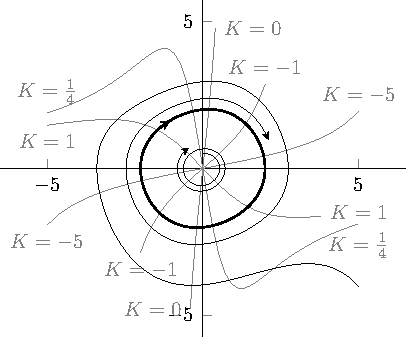
\includegraphics{figSystemVanDerPolEquationA}
\caption{ون ڈر پول مساوات؛ \عددی{0.1} لیتے ہوئے دو خط حرکت کو تحدیدی گردش تک پہنچتے ہوئے دکھایا گیا ہے۔}
\label{شکل_نظام_ون_ڈر_پول_پہلی_شکل}
\end{figure}
%
\begin{figure}
\centering
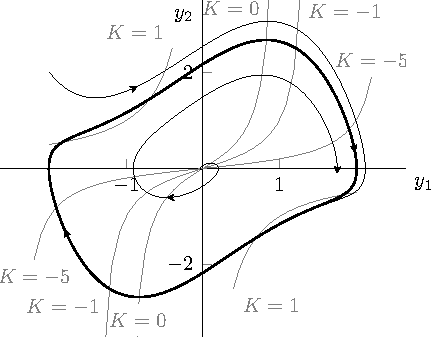
\includegraphics{figSystemVanDerPolEquationB}
\caption{ون ڈر پول مساوات؛ \عددی{1} لیتے ہوئے دو خط حرکت کو تحدیدی گردش تک پہنچتے ہوئے دکھایا گیا ہے۔}
\label{شکل_نظام_ون_ڈر_پول_دوسری_شکل}
\end{figure}
\انتہا{مثال}
%=====================

